% % % % % % % % % % % % % % % % % % % % % % % % % % % % % % % % % %
%\documentclass[runningheads]{llncs}
%\documentclass[12pt,letterpaper]{article}
%\documentclass[preprint,12pt]{elsarticle}
%\documentclass{sig-alternate}
\documentclass[10pt,preprint,nonatbib]{sigplanconf}

% https://avandeursen.com/2013/07/10/research-paper-writing-recommendations/


% packages
\usepackage{xspace}
\usepackage{ifthen}
\usepackage{amsbsy}
\usepackage{amssymb}
\usepackage{balance}
\usepackage{alltt} 
\usepackage{booktabs}
\usepackage{graphicx}
\usepackage{multirow}
\usepackage{needspace}
\usepackage{microtype}
\usepackage{bold-extra}
\usepackage{adjustbox}
\usepackage{subfig}
\usepackage{wrapfig}
\usepackage{balance}
\usepackage[colorlinks]{hyperref}
\usepackage[all]{hypcap}
\usepackage{xcolor}
\usepackage{textcomp}
\usepackage{listings}
\definecolor{source}{gray}{0.9}
\setcounter{tocdepth}{2}

\def\chapterautorefname{Chapter}
\def\appendixautorefname{Appendix}
\def\sectionautorefname{Section}
\def\subsectionautorefname{Section}
\def\figureautorefname{Figure}
\def\tableautorefname{Table}
\def\listingautorefname{Listing}

\lstset{
	language={},
	% characters
	tabsize=3,
	upquote=true,
	escapechar={!},
	keepspaces=true,
	breaklines=true,
	alsoletter={\#:},
	breakautoindent=true,
	columns=fullflexible,
	showstringspaces=false,
	basicstyle=\footnotesize\sffamily,
	% background
	frame=single,
    framerule=0pt,
	backgroundcolor=\color{source},
	% numbering
	numbersep=5pt,
	numberstyle=\tiny,
	numberfirstline=true,
	% captioning
	captionpos=b,
	% formatting (html)
	moredelim=[is][\textbf]{<b>}{</b>},
	moredelim=[is][\textit]{<i>}{</i>},
	moredelim=[is][\color{red}\uwave]{<u>}{</u>},
	moredelim=[is][\color{red}\sout]{<del>}{</del>},
	moredelim=[is][\color{blue}\underline]{<ins>}{</ins>}}
\newcommand{\ct}{\lstinline[backgroundcolor=\color{white},basicstyle=\small\ttfamily]}
\newcommand{\lct}[1]{{\small\tt #1}}

% proof-reading
\usepackage{xcolor}
\usepackage[normalem]{ulem}
\newcommand{\ra}{$\rightarrow$}
\newcommand{\ugh}[1]{\textcolor{red}{\uwave{#1}}} % please rephrase
\newcommand{\ins}[1]{\textcolor{blue}{\uline{#1}}} % please insert
\newcommand{\del}[1]{\textcolor{red}{\sout{#1}}} % please delete
\newcommand{\chg}[2]{\textcolor{red}{\sout{#1}}{\ra}\textcolor{blue}{\uline{#2}}} % please change
\newcommand{\chk}[1]{\textcolor{ForestGreen}{#1}} % changed, please check

% comments \nb{label}{color}{text}
\newboolean{showcomments}
\setboolean{showcomments}{true}
\ifthenelse{\boolean{showcomments}}
	{\newcommand{\nb}[3]{
		{\colorbox{#2}{\bfseries\sffamily\scriptsize\textcolor{white}{#1}}}
		{\textcolor{#2}{\sf\small$\blacktriangleright$\textit{#3}$\blacktriangleleft$}}}
	 \newcommand{\version}{\emph{\scriptsize$-$Id$-$}}}
	{\newcommand{\nb}[3]{}
	 \newcommand{\version}{}}
\newcommand{\rev}[2]{\nb{Reviewer #1}{red}{#2}}
\newcommand{\ab}[1]{\nb{Alexandre}{blue}{#1}}
\newcommand{\lr}[1]{\nb{Lukas}{pink}{#1}}
\newcommand{\ai}[1]{\nb{Alejandro}{orange}{#1}}
\newcommand{\on}[1]{\nb{Oscar}{olive}{#1}}


% graphics: \fig{position}{percentage-width}{filename}{caption}
\DeclareGraphicsExtensions{.png,.jpg,.pdf,.eps,.gif}
\graphicspath{{figures/}}
\newcommand{\fig}[4]{
	\begin{figure}[#1]
		\centering
		\includegraphics[width=#2\textwidth]{#3}
		\caption{\label{fig:#3}#4}
	\end{figure}}

\newcommand{\largefig}[4]{
	\begin{figure*}[#1]
		\centering
		\includegraphics[width=#2\textwidth]{#3}
		\caption{\label{fig:#3}#4}
	\end{figure*}}
	
\newcommand{\wrapfig}[5]{	
\begin{wrapfigure}{#1}{#2\textwidth}
  \begin{center}
    \includegraphics[width=#3\textwidth]{#4}
  \end{center}
  \caption{\label{fig:#4}#5}
\end{wrapfigure}}

% abbreviations
\newcommand{\ie}{\emph{i.e.,}\xspace}
\newcommand{\eg}{\emph{e.g.,}\xspace}
\newcommand{\etc}{\emph{etc.}\xspace}
\newcommand{\etal}{\emph{et al.}\xspace}

% lists
\newenvironment{bullets}[0]
	{\begin{itemize}}
	{\end{itemize}}

\newcommand{\seclabel}[1]{\label{sec:#1}}
\newcommand{\figlabel}[1]{\label{fig:#1}}
\newcommand{\tablabel}[1]{\label{tab:#1}}
\newcommand{\figref}[1]{Figure~\ref{fig:#1}}
\newcommand{\secref}[1]{Section~\ref{sec:#1}}


%Specialized macros
\pagenumbering{arabic}
\DeclareCaptionType{copyrightbox}
\newcommand{\myparagraph}[1]{\vspace{0.1cm}\noindent \textbf{\textit{#1.}}}



\balance

% constants
% \newcommand{\Title}{Toward Reducing Waste of Expandable Collections: The Pharo Case}
\newcommand{\Title}{Accurate VM profiler for the Cog VM}
%\newcommand{\Title}{The Dark Side of Expandable Collections: The Pharo Case}
\newcommand{\TitleShort}{\Title}
%\newcommand{\Authors}{~~~~}
\newcommand{\Authors}{Sophie Kaleba, Cl\'ement B\'era, Alexandre Bergel$^3$\\[2 ex]
$^3$Pleiad Lab, DCC, University of Chile}
\newcommand{\AuthorsShort}{}

\hypersetup{
	colorlinks=true,
	urlcolor=black,
	linkcolor=black,
	citecolor=black,
	plainpages=false,
	bookmarksopen=true,
	pdfauthor={\Authors},
	pdftitle={\Title}}
	
\newenvironment{code}
    {\begin{alltt}\sffamily}
    {\end{alltt}\normalsize}	
	
%\newcommand{\Authors}{Alexandre Bergel, Vanessa Pe\~na}
%\newcommand{\AuthorsShort}{A. Bergel, V. Pe\~na}

%\journal{Science of Computer Programming}

% \makeatletter
% \let\@copyrightspace\relax
% \makeatother
% 

%double spaced
%\renewcommand{\baselinestretch}{1.5}

\begin{document}

\special{papersize=8.5in,11in}
\setlength{\pdfpageheight}{\paperheight}
\setlength{\pdfpagewidth}{\paperwidth}

\conferenceinfo{OOPSLA '14}{Month d--d, 20yy, City, ST, Country}
\copyrightyear{2014}
\copyrightdata{978-1-nnnn-nnnn-n/yy/mm}
\doi{nnnnnnn.nnnnnnn}


%\begin{frontmatter}
\title{\Title}


\authorinfo{Sophie Kaleba$^1$, Cl\'ement B\'era$^1$, Alexandre Bergel$^2$, St\'ephane Ducasse$^1$}
           {$^1$INRIA- Lille Nord Europe, France\\
             $^2$Pleiad Lab, DCC, University of Chile, Santiago, Chile}
           {}
%\author{\Authors
%}


%\institute{~~}
%\institute{Pleiad Lab, University of Chile}
\maketitle

\begin{abstract}

%context
Code profiling enables a user to know where in an application or function the execution time is spent. The Pharo ecosystem offers several code profilers. However, most of the publicly available profilers (MessageTally, Spy, GadgetProfiler) largely ignore the activity carried out by the virtual machine, thus incurring inaccuracy in the gathered information and missing important information, such as the Just-in-time compiler activity.

This paper motivates and describes the latest innovations carried out in VMProfiler, a code execution profiler hooked into the virtual machine, that exercises its analysis by monitoring the virtual machine execution. These innovations address some limitations related to assessing the activity of native functions (resulting from a Just-in-time compiler operation): VMProfiler now provides accurate profiling reports, showing for large native code functions in which bytecode range the execution time is spent.

%Profiling tools are already available for Smalltalk-based languages, like MessageTally, GadgetProfiler or VMProfiler. The latter, especially, by tracking down where the time is spent on the virtual machine (VM) side, can provide significant data to help tuning the VM settings for performance.
%
%%problem
%However, while this VM profiler can identify in which functions the execution time is spent, it cannot identify where in these functions the time is spent. This is getting critical as the optimisations performed by the Just-In-Time compiler (JIT) result in functions of greater size, which are then harder to profile accurately.
%
%%solution
%In this paper, we discuss this problem and then we introduce the solution proposed to keep collecting relevant profiling data, using an API that allow us to identify, for a given function, in which bytecode range the time is spent.

\end{abstract}

%\begin{keyword}
%% keywords here, in the form: keyword \sep keyword

%% MSC codes here, in the form: \MSC code \sep code
%% or \MSC[2008] code \sep code (2000 is the default)
%profiling \sep virtual machine \sep cog
%\end{keyword}




%\end{frontmatter}
%: % % % % % % % % % % % % % % % % % % % % % % % % % % % % % % % % %

\section{Introduction}

%TEMPLATE:
%
%Context
%
%Problem
%
%Known tracks for \sd{solutions}
%	here you want to show that you are not an idiot not knowing what have been around
%
%What our solution is \ct{Set} and \ct{OrderedCollection} (so that the reader knows where the paper is going)
%
%Contribution of the paper
%
%Paper structure


%context
%main challenge in general and thus for VMs: performance

Although computers tend to get more and more powerful, performance, especially in terms of execution time, remains a major goal to be pursued. This statement applies of course to virtualised environments and assuring the performance of the \textbf{v}irtual \textbf{m}achine (VM) is critical when you aim for an overall good performance. 
Thus, it is crucial to know where the time is spent in the VM during execution: indeed, it helps identifying where to tune its settings to actually get better results.

To get a precise idea of the program behavior, critical information can be collected by profiling code.
Such profiling tools are already available in Pharo, like MessageTally \cite{Berg13a} and VMProfiler \cite{Mira08b}: they provide statistical/graphical reports, showing the methods in which most of the execution time is spent, and how much of this time is spent in garbage collection \cite{Berg13a}. However, the VM profiler, unlike MessageTally, provides statistical data about the time spent in the Cog VM. Cog~\cite{Mira08a}~ is a virtual machine designed for Smalltalk, and currently used for various Smalltalk-based languages such as Pharo~\cite{Blac09a} or Squeak~\cite{Blac07a}. It features a bytecode interpreter and a \textbf{j}ust-\textbf{i}n-\textbf{t}ime compiler (JIT). It is in the code of these features that we find out where the execution time is spent.\\

% problem 
Right now, VMProfiler cannot track down precisely where the time is spent when executing the code generated by the JIT. It can track down in which methods the time is spent, but it cannot track down in which part of those methods the time is spent. For example, assuming there is a frequently used method with multiple loops, VMProfiler mentions that most of the time is spent in this method (it is indeed frequently used), but it cannot mention in which loop the time is spent.

This problem is more and more significant as new optimisations are added to the JIT, based on the work of H\"olzle and Ungar~\cite{Holz94a}. The development branch of the JIT now features speculative inlining. In this context, the JIT generates a single machine code method for multiple unoptimised bytecode methods (the method optimised and the inlined methods). The VM profiler shows that most of the time is spent in optimised code, but it is currently not possible to know in which inlined method most of the time is spent. So while we get a faster and more performant VM, we cannot tune the JIT for performance.\\

%solution
To get accurate profiling data again, VMProfiler has to be enhanced to show specifically where the time is spent in a method. To do so, we use the API usually used for debugging, that maps machine code program counter (pc) to bytecode program counter. This way, we can tell for each method appearing in the report in which bytecode range most of the time is spent.\\

In this paper, we will first discuss about the existing VMProfiler, and how the inaccuracy of its reports raises a problem when large native code functions are profiled. Then, we describe the proposed solution to address this problem. Eventually, we mention other profiling tools in Smalltalk and other programming languages and compare them against VMProfiler.


%: % % % % % % % % % % % % % % % % % % % % % % % % % % % % % % % % %

\section{Accurate profiling of jitted code}

This section first defines the terminology used in the paper, then describes the existing VMProfiler available in the Cog VM clients such as Squeak or Pharo, and the debugger mapping and lastly states the problem analysed in the rest of the paper.

\subsection{Terminology}

\paragraph{Function.} In the paper, we use the term \emph{function} to refer to executable code, in our case, method or block closures.

\paragraph{Bytecode function.} The term \emph{bytecode function} is used to refer specifically to the compiled function in the form of bytecode, for example, instances of \ct{CompiledMethod} in the case of methods. Bytecode functions are regular objects accessible from the Squeak/Pharo runtime and are present in the heap with all other objects. These functions are executable by the VM.

\paragraph{Native function.} We use the term \emph{native function} to refer to the representation of a function generated by Cog's JIT, which includes the native code. Native functions are not regular objects and are allocated in a specific memory zone (called the \emph{machine code zone}), which is executable. These functions are executable by the processor.

\subsection{Existing VM profiler}

VMProfiler has been available for almost a decade in Squeak and has been recently ported to Pharo. VMProfiler allows one to track down where the time is spent in the VM when executing a specific portion of code. VMProfiler computes where the time is spent in the compiled C code of the VM, in the VM plugins and in the native functions. All the results are available as a statistical report. A typical report includes two main sections, the time spent in generated code, \ie in native functions and the time spent in the compiled C code. The time spent in the compiled C code includes the time spent in the bytecode interpreter, in the garbage collector and in the JIT. 
 
\paragraph{Cog memory.} As depicted in \figref{CogMemory}, the machine code zone is composed of three areas (in order, the numbers match the numbers on the figure):
\begin{enumerate}
	\item The first area includes all the trampolines and enilmoparts generated at VM start-up. Trampolines are native code routines. Some of them are used as discovery routine at VM start-up to know which instructions the processor supports. The other trampolines are called from native functions, either to switch to the C runtime of the VM or just to execute specific uncommon code. Enilmoparts (trampoline written backward) are native code routines called from the C runtime of the VM to switch to native functions generated by the JIT. 
	\item The second area is composed of native functions (CogMethods or CogFullBlocks, depending if a method or a block closure is compiled) and \textbf{p}olymorphic \textbf{i}nline \textbf{c}aches (PIC) (ClosedPICs, PICs represented as a jump table up to 6 cases or OpenPICs, PICS represented as a hash map search with a 8 entry hash map).~\cite{Holz91a}
	\item The last area is a linked list of native functions or PICs referencing young objects. This list is used by the scavenger.
\end{enumerate}

\begin{figure}[htp!]
     \begin{center}
         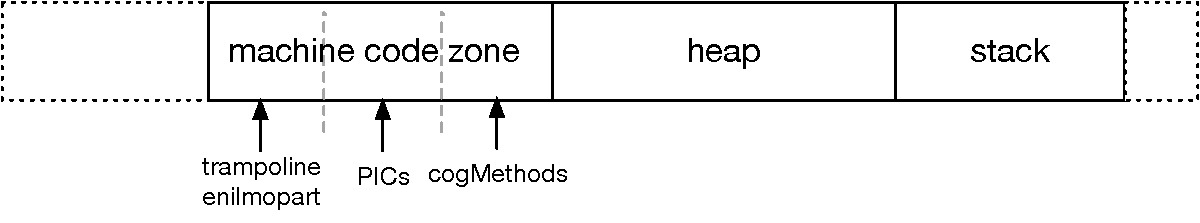
\includegraphics[width=\linewidth]{CogMemory}
         \caption{Machine code zone layout}
         \label{fig:CogMemory}
     \end{center}
 \end{figure}

During the runtime, part of the machine code zone is unused. When the machine code zone is full and a new function needs to be compiled, a code compaction happens, freeing a quarter of the machine code zone, using a least recently used naive algorithm. Hence, while running a normal application, up to a quarter of the machine code zone is free. 

We use three keywords to identify different addresses in the machine code zone. \emph{CogCode} is the beginning of the machine code zone, before the trampolines and enilmoparts. \emph{CCFree} is the beginning of the unused part of the machine code zone. \emph{CCEnd} is the last address of the machine code zone before the linked list of young referrers.

\paragraph{Implementation.} Implementation-wise, VMProfiler is a sampling profiler. When profiling is started, a separate high-priority OS thread is started and collects the instruction pointers of the VM OS thread in a large circular buffer at an approximate cadence of 1.4GHz. Once profiling stops, a primitive method is available to gather the samples from the VM into a Bitmap. To understand to which functions the samples correspond to, VMProfiler requests:
\begin{itemize}
	\item The symbol table of the VM executable and all external plugins.
	\item A description of the native functions currently present in the machine code zone.
\end{itemize}
Each function (indifferently, a native function or a C function) is represented as a function symbol (the name of the function, either the Smalltalk function name with the method class and the selector or the C function symbol), a start address and the last address. VMProfiler uses these ranges to find out in which function each profiling sample is, as shown in \figref{fig:OriginalMapping}. Then, the profiler generates a report, either in the form of a string or through a user interface.

 \begin{figure}[t!]
     \begin{center}
         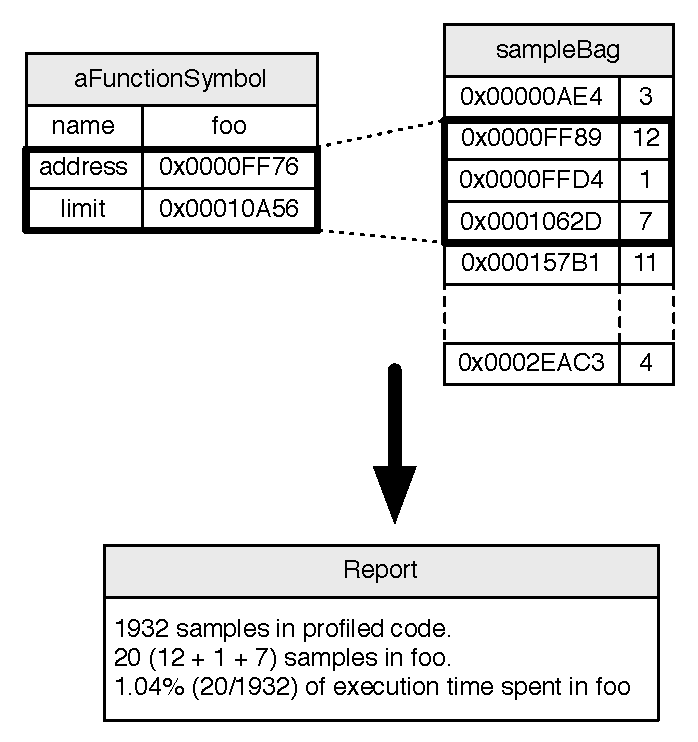
\includegraphics[width=0.85\linewidth]{OriginalMapping}
         \caption{Mapping in original code}
         \figlabel{fig:OriginalMapping}
     \end{center}
 \end{figure}
 
 \paragraph{Primitive Cog Constituents.}
The primitive \ct{primitive CollectCogCodeConstituents} provides VMProfiler with the description of the native functions currently present in the machine code zone it needs. 
This primitive answers an array of pair-wise elements as shown in \figref{fig:ContentsOfCollectCogCodePrim}. The first element of the pair is either :
\begin{itemize}
	\item the name of a trampoline/enilmopart
	\item a function pointer
	\item the name of a selector (for PICs)
	\item annotations (\ie CCFree, CCEnd)
\end{itemize}
The second item of the pair is the start address of this element in the machine code zone.

\ct{primitiveCollectCogCodeConstituents} is called once the profiling samples has been gathered. These samples will be mapped with the data answered by the primitive. For instance, if a sample is equal to \ct{0x89012F0}, one can find out it refers to \ct{Behavior>>new} thanks to the primitive, as showed in \figref{fig:ContentsOfCollectCogCodePrim}.

 \begin{figure}[b!]
     \begin{center}
         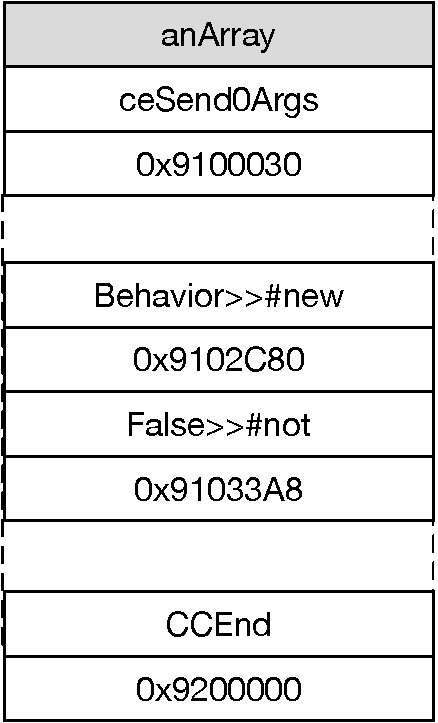
\includegraphics[width=0.66\linewidth]{ContentsOfCollectCogCodePrim}
         \caption{Cog constituents as answered by the primitive}
         \figlabel{fig:ContentsOfCollectCogCodePrim}
     \end{center}
 \end{figure}
 
\subsection{Debugger mapping}

To be able to debug native functions as if they were executed as bytecode functions by the bytecode interpreter, when Cog's JIT generates a native function for a given bytecode function, it generates a list of annotations~\cite{Ber16d} allowing one to reconstruct the interpreter state of the function activation at any point where the code execution can be interrupted (message sends, conditional branches or back jumps). Each annotation includes a mapping between the pc in the machine code and the pc in the bytecode of the method. The VM is able to use these annotations to reify function activations and provide it to Pharo.
 
\subsection{Problem}

The VM development team is currently working on the implementation of an optimising JIT for the Cog VM. These optimisations includes speculative inlining, as described in the work of H\"olzle and Ungar~\cite{Holz94a}, in a similar way to production VMs such as Java's hotspot VM (The hotspot VM is the default virtual machine for Java~\cite{Pale01a}) and Javascript's V8 engine (V8 is mostly used as the Javascript engine for Google Chrome and NodeJS.~\cite{V8}). The optimising JIT is designed as a bytecode functions to bytecode functions runtime optimising compiler, re-using the existing JIT as a back-end to generate native functions. In this context, optimised functions are present both in the form of bytecode functions and native functions, using the extended bytecode set described in the work of B\'era \etal~\cite{Bera14a}. When profiling optimised code for benchmarks such as the Games benchmark~\cite{GameBenchs}, VMProfiler now shows that all the time is spent in a single function (the function where the rest of the functions used by the benchmark are inlined). To improve performance and tune the optimising JIT, the VM development team requires more information about where the time is spent in optimised functions, for example, in which range of bytecodes the time is spent.

\vspace{0.2cm}
\paragraph{Problem statement.} \emph{How to provide accurate profiling information in large native functions profiled?}
\vspace{0.2cm}

To address this problem, we propose an implementation that takes advantage of an API used for debugging, to map machine code pc to bytecode pc, to be able to identify in which bytecode range the time is spent in a function. The implementation is specific to the Cog VM, with a working version in both Squeak and Pharo. A similar design could apply in other VMs featuring similar debugging capabilities.

%: % % % % % % % % % % % % % % % % % % % % % % % % % % % % % % % % %

\section{Solution}

To profile accurately large native functions, we re-use the API available for debugging to identify in which section of the function the time is spent. The solution is split in two steps. First, we enhanced the primitive providing the description of the native functions present in the machine code zone to provide a mapping between machine code pc and bytecode pc in addition to the start address of the function. Second, we used the mapping to identify in which range of bytecodes each sample is.

\subsection{Improved primitive}

In the improved version of the primitive, if the native function has at least one machine code pc mapped to a bytecode pc, the primitive answers for the function, instead of the start address, an array starting with the start address followed by pairs of machine code pc and the corresponding mapped bytecode pc. 

For example, the function \ct{foobarbaz} in \figref{Code} sends 3 messages. Once translated to bytecode, there are indeed 3 send bytecodes, each responsible for the sending of a message (on bytecode pc 26, 29 and 32, in bold in \figref{Example}). For this function, the existing primitive was answering 2 elements: the pointer to the native function and its start address in the machine code zone

\begin{figure}[h!]
    \begin{center}
    	\begin{tabular}{l@{\hspace{1cm}}@{\hspace{1cm}}l}
    		\underline{\textbf{Source code}} & \underline{\textbf{Bytecode}} \vspace{0.2cm} \\
		foobarbaz & 25 \textless4C\textgreater~self \\
    		\hspace{0.5cm} self foo. & \textbf{26 \textless80\textgreater~send: foo} \\
    		\hspace{0.5cm} self bar. & 27 \textless{D8}\textgreater~pop \\
    		\hspace{0.5cm} self baz. & 28 \textless4C\textgreater~self \\
        		& \textbf{29 \textless81\textgreater~send: bar} \\
        		& 30 \textless{D8}\textgreater~pop\\
        		& 31 \textless4C\textgreater~self\\
        		& \textbf{32 \textless82\textgreater~send: baz}\\
        		& 33 \textless{D8}\textgreater~pop\\
        		& 34 \textless58\textgreater~returnSelf\\
	\end{tabular}
	\caption{Example method}
    \label{fig:Code}
    \end{center}
\end{figure}

As you can see in \figref{BytecodeRange}, the improved primitive still answers 2 elements, but, while the first one remains unchanged and still refers to the name of the function, the second one is an array, because the 3 send bytecodes are mapped. The first element of this array is the starting address of the function in the machine code zone. The other elements come by pair: the first one is the machine code pc, the second one is the bytecode pc.
The results answered by the improved primitive are then used to determine bytecode ranges in the function. In \figref{BytecodeRange}, there are 4 bytecode ranges, each delimited by a mapped bytecode pc.  

%\begin{itemize}
%	\item TO CHANGE WITH FIGURE
%	\item 0x0000FF45-47 - bc 1 to bc 26
%	\item 0x0000FF47-52 - bc 26 to bc 29
%	\item 0x0000FF52-63 - bc 29 to bc 32
%	\item 0x0000FF63-end - bc 32 to bc 34
%\end{itemize}

 \begin{figure}[htp!]
     \begin{center}
         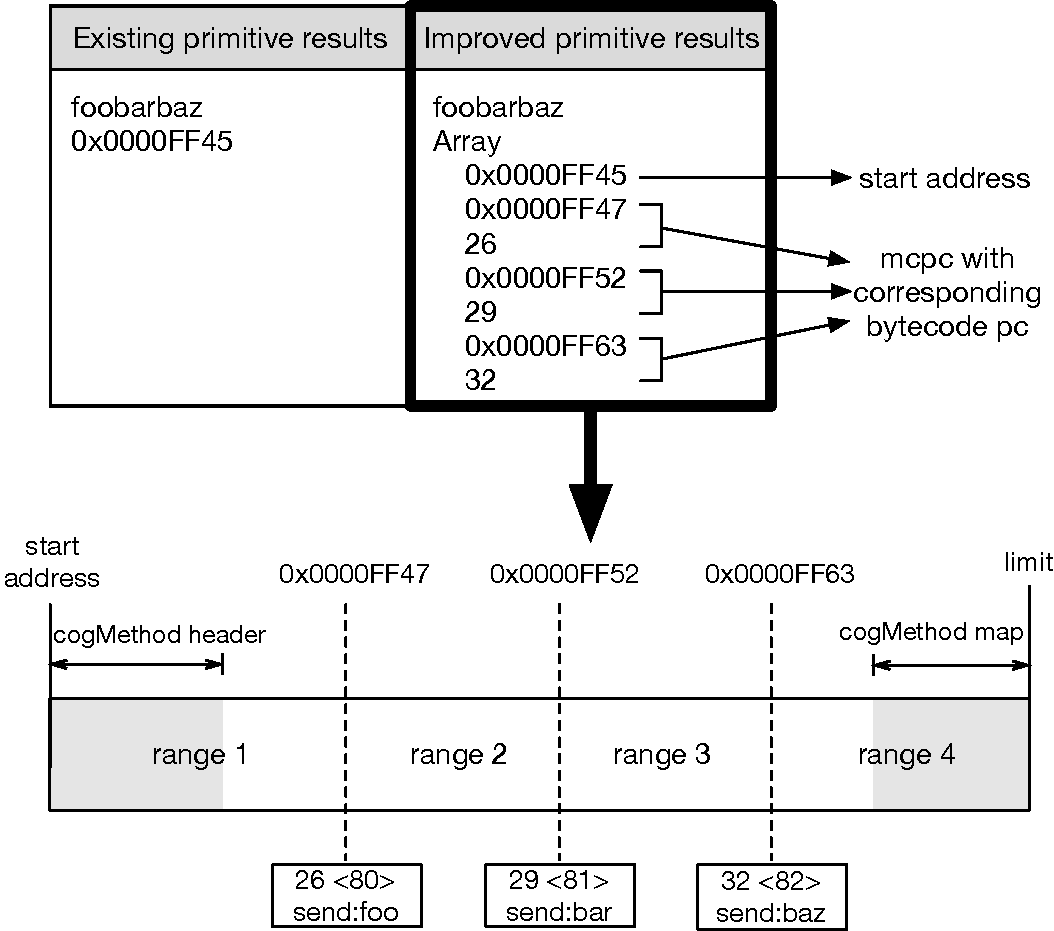
\includegraphics[width=1.0\linewidth]{BytecodeRange}
         \caption{Example of primitive results}
         \label{fig:BytecodeRange}
     \end{center}
 \end{figure}


%\begin{figure}[h!]
%    \begin{center}
%		\noindent  \begin{tabular}{l | l}
%		TO CHANGE \small Existing primitive result & \small Improved primitive result \\		
%		\midrule
%		foobarbaz & foobarbaz \\
%		0x0000FF45 & anArray containing: \\
%		& 0x0000FF45 \\
%		& 0x0000FF47 \\
%		& 26 \\
%		& 0x0000FF52 \\
%		& 29 \\
%		& 0x0000FF63 \\
%		& 32 \\\
%		0x0000FF45 & anArray containing: \\
%		& 0x0000FF45 \\
%		& 0x0000FF47 \\
%		& 26 \\
%		& 0x0000FF52 \\
%		& 29 \\
%		& 0x0000FF63 \\
%		& 32 \\
%
%		\end{tabular}
%	\caption{Example of primitive results\label{fig:Primitive}}
%    \end{center}
%\end{figure}

\subsection{Accurate mapping and report}

To compute the profiling statistics, the profiler uses the primitive to create a description of the native functions currently present in the machine code zone.  Each function is represented by a functionSymbol object, characterized by the name of the function and its starting and limit addresses in the machine code zone.
A new field in \ct{FunctionSymbol} has been added to take the results of the modified primitive into account: \textit{mcpcbcpcmap}, standing for machine code program counter - bytecode program counter map. This dictionary associates a machine code pc with a bytecode pc.

As shown in \figref{NewMapping}, this new field helps with identifying where the execution time is spent. For instance, we know that \ct{foobarbaz} starts at \ct{0x0000FF45}, and that the first mapped bytecode pc (26) is at \ct{0x0000FF47}: it means that the 12 samples within this address range will refer to the bytecode instructions between 1 and 26.
The same applies for the other entries: the unique sample within the range \ct{0x0000FF47} and \ct{0x0000FF52} will refer to the bytecode instructions between 26 and 29. 

In that case, 1932 samples were gathered in total and 20 were referring to \ct{foobarbaz}. Among these 20 samples, 12 were referring to foo's bytecode pc between 1 and 26. Therefore, 60\% of the time spent in \ct{foobarbaz} was spent between these bytecode pc.


 \begin{figure}[!htp]
     \begin{center}
         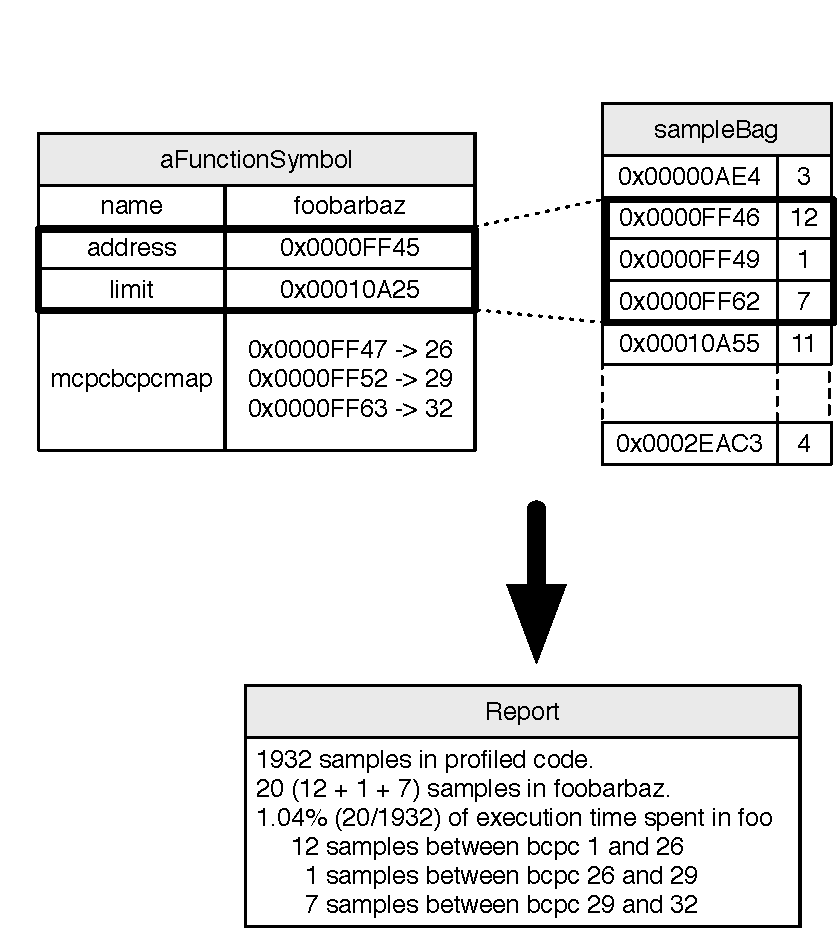
\includegraphics[width=1.0\linewidth]{NewMapping}
         \caption{Mapping with new feature}
         \label{fig:NewMapping}
     \end{center}
 \end{figure}
 
%: % % % % % % % % % % % % % % % % % % % % % % % % % % % % % % % % %

\section{Example}

  \begin{figure*}[!htp]
     \begin{center}
         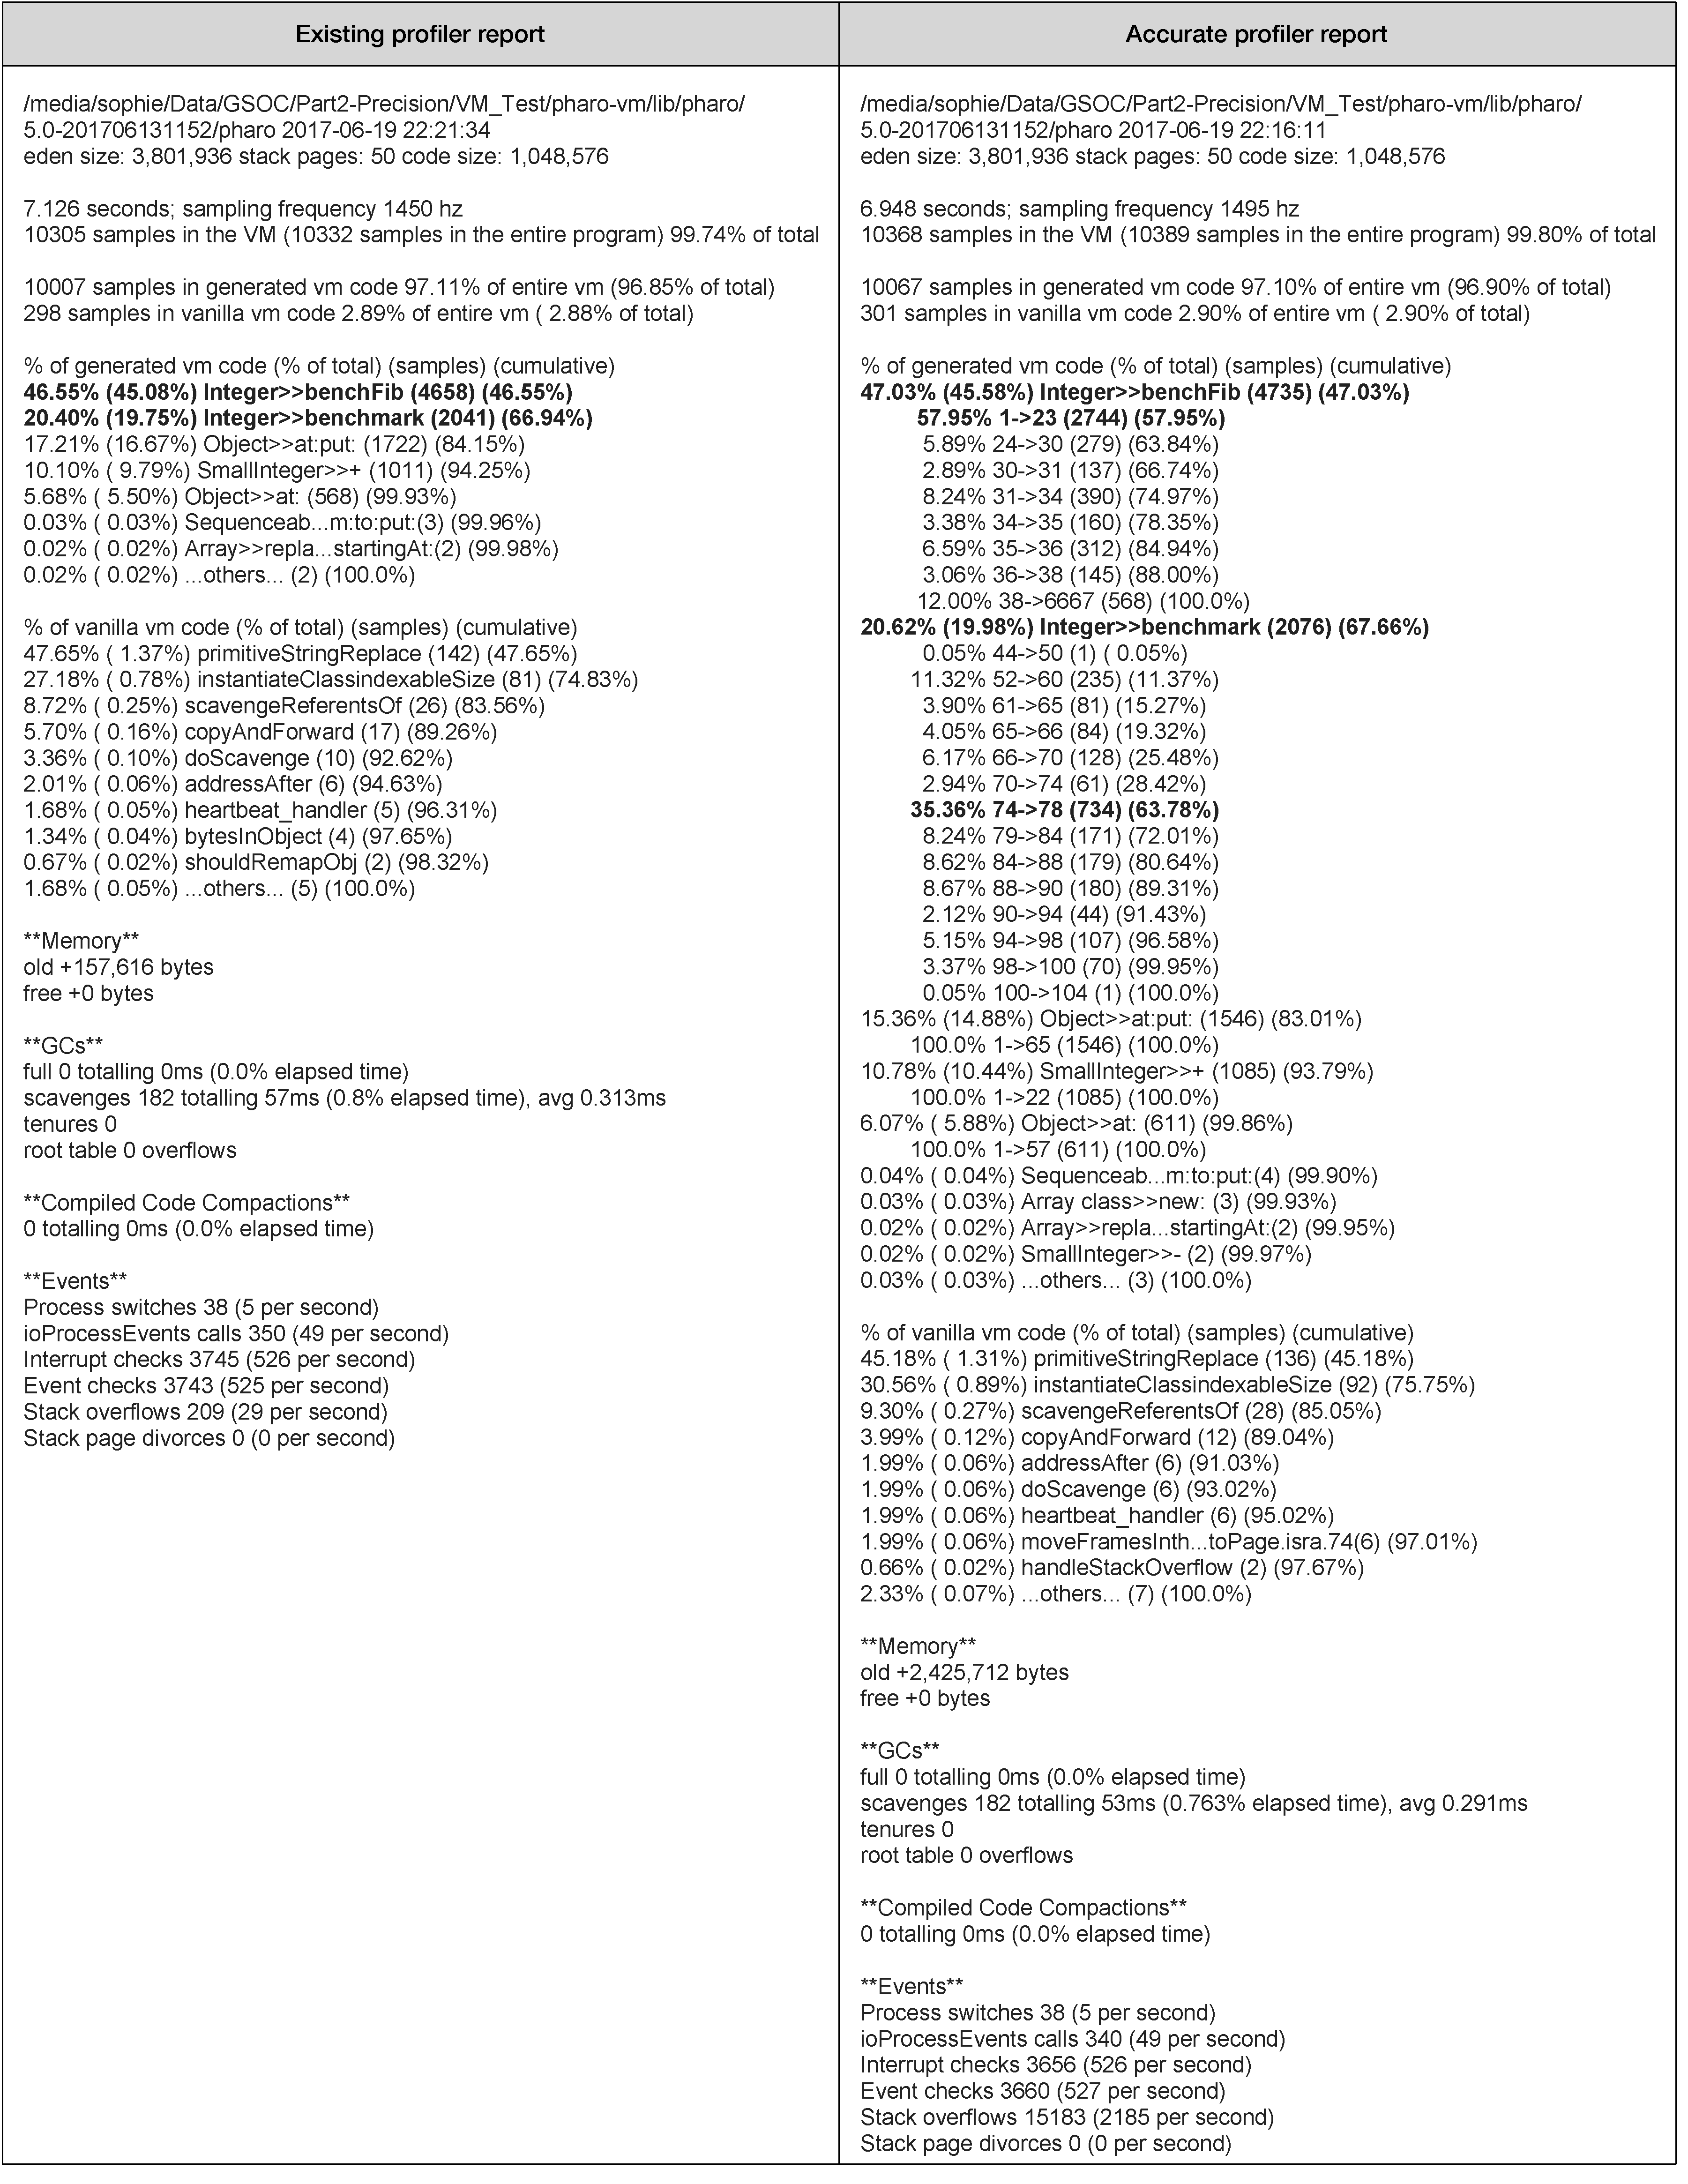
\includegraphics[width=1.0\linewidth]{ReportComparison}
         \caption{Comparison of profiling reports for \ct{10 tinyBenchmark}}
         \figlabel{fig:ReportComparison}
     \end{center}
 \end{figure*}

In this section, we present a concrete example of profiling on a benchmark.

We profiled the following benchmark: \ct{10 tinyBenchmarks} using first the existing VMProfiler, and using then the accurate VMProfiler. 
\figref{fig:ReportComparison} puts the two profiling reports side by side.
Among the jitted methods, \ct{Integer>>benchFib} was the one in which most of the execution time was spent (around 45\% of the total time).

In the existing version of the profiler, one cannot identify where those 45\% of the total execution time are spent. In the accurate version, however, the method is decomposed in several bytecode ranges (in this case, 8): one can then identify in which bytecode range(s) most of the time is spent. Here, 57,95\% that time is spent in the entry. The next significant part of time is spent in the last bytecode instructions (12\% starting from bytecode pc 38).

In the \ct{Integer>>benchmark} function, most of the time is spent in the 74 -$>$ 78 bytecode range, referring to the following bytecode instructions: 
\begin{itemize}
	\item \ct{75 <6B> popIntoTemp: 3}
	\item \ct{76 <13> pushTemp: 3}
	\item \ct{77 <10> pushTemp: 0}
	\item \ct{78 <B4> send: <=}
\end{itemize}
The \ct{90 <A3> jumpTo: 76} instruction indicates that there is a loop between the 76 and 90 bytecode instructions. Thus, we can assume that the time is mostly spent in the 76, 77 and 78 bytecode instructions.

%: % % % % % % % % % % % % % % % % % % % % % % % % % % % % % % % % %
\section{Related Work}\seclabel{relatedWork}

The field of execution profiling is vast and has received a large attention from the research community. This section presents the different works related to the effort presented in this paper.

\subsection{Standard Pharo profilers}

Smalltalk, and therefore Pharo, offers a sophisticated reflective API. Threads are openly exposed and the stack for each active thread may be introspected. In addition, the next thread in the execution queue may be accessed. \ct{MessageTally} and \ct{AndreasSystemProfiler} are two standard profilers in Pharo that exploit this advanced reflective API. Both follow the same principle: a thread of high-priority is run and regularly it samples the thread queue. The frequency of the samples typically ranges from 1 to 10 milliseconds. After the program execution, frequency of method context frames is determined. Such frequency is used to estimate the time spent in each frame. 

Both profilers essentially rely on the Smalltalk reflective API. Since most of the computation happens within the image, the overhead of the profiler is therefore likely to be expensive and intrusive (\eg time to execute an application is longer when being profiled). It is known that getting a sample profiler with a high-precision is difficult to achieve and prone to error~\cite{Mytk08a,Mytk10a,Berg11d}. 

%====
\subsection{Support in the Virtual Machine}

The Java Virtual Machine Tool Interface (JVM TI) is a native programming interface offered by the JVM to build dedicated profiling and debugging tools\footnote{\url{https://docs.oracle.com/javase/8/docs/platform/jvmti/jvmti.html}}. JVM TI provides both a way to inspect the state and to control the execution of Java applications. %JVM TI is a two-way interface

A JVM TI client, defined as an \emph{agent}, can be notified of particular events emitted by the JVM. In total, a client may receive 31 different kinds of JVM events. These events cover breakpoints, class loading, garbage collection, method execution, monitor, and virtual machine start up and destruction.

JVisualVM\footnote{\url{https://visualvm.github.io}} is a visual profiling tool and framework. JVisualVM offers a large set of features, including remote debugging / profiling, thread analysis, heap snapshot, and garbage collection monitoring. 

%====
\subsection{Generic profilers}

The profiling tool described in this paper is intended to be used to address performance issues. The software engineering community has produced software execution monitoring technique to profile various aspects related to an execution~\cite{Ress12a,Ress12b}. 

A common profiling technique is to use instrumentation instead of sampling~\cite{Metz05a}. For example, Spy~\cite{Berg11h} is a framework to build domain-specific profilers, with application ranging from memory consumption analysis~\cite{Infa15a} to test coverage~\cite{Berg12c}.


%: % % % % % % % % % % % % % % % % % % % % % % % % % % % % % % % % %
\section{Conclusion and Future Work}\seclabel{conclusion}

In this paper, we have presented the evolutions carried out in VMProfiler, a profiler enabling to identify where the execution time is spent in the VM side, i.e. identify where the time is spent in the C code of the VM (interpreter, garbage collector) and in the jitted functions.

As this kind of tool is typically used to know where to boost performance, the existing VMprofiler could be improved: it could not provide accurate profiling data for large native code functions. Indeed, it could report that most of the execution time was spent in a function, but not \textit{where} in this function the time was spent.
This problem was getting significant as more and more optimisations were performed by the JIT ; inlining, especially, makes the jitted functions larger, and thus, harder to accurately profile.

This paper describes a way to address this problem : an API used for debugging purposes offers a mapping between machine code pc and bytecode pc. This mapping is then used to determine bytecode ranges in a large native code function, and thus identifies how many samples are included in one or the other range. Now, VMProfiler provides accurate profiling statistical reports. \\

Further improvements are currently being considered: 
\begin{itemize}
	\item As for now, VMProfiler is only available headless in Pharo. A graphical user interface could be implemented to provide profiling data from another perspective.
	\item Sometimes, customers in a Windows environment request profiling, yet the VMProfiler is currently available for Mac and Linux only. The VMProfiler could then be implemented for Windows to tackle this problem.
	\item Currently, VMProfiler shows PIC disregarding if the PIC is a closed PIC or an open PIC. It would be nice to extend it to show this information (it requires changes in \ct{primitiveCollectCogCodeConstituents}).
\end{itemize}


\section*{Acknowledgments}
We thank Eliot Miranda for the original implementation of VMProfiler and his support during the evolution.
[+ ajouter le reste]
%: % % % % % % % % % % % % % % % % % % % % % % % % % % % % % % % % %

%{\small
\bibliographystyle{alpha}
\bibliography{sista,rmod,others}
%\bibliography{hapao}
%}


%\appendix 
\end{document}

